\section{Zukunft}

\begin{frame}{Aussichten}
    \begin{columns}
        \begin{column}{0.5\textwidth}
            Aber erst ein Blick zurück
            \begin{figure}
                \centering
                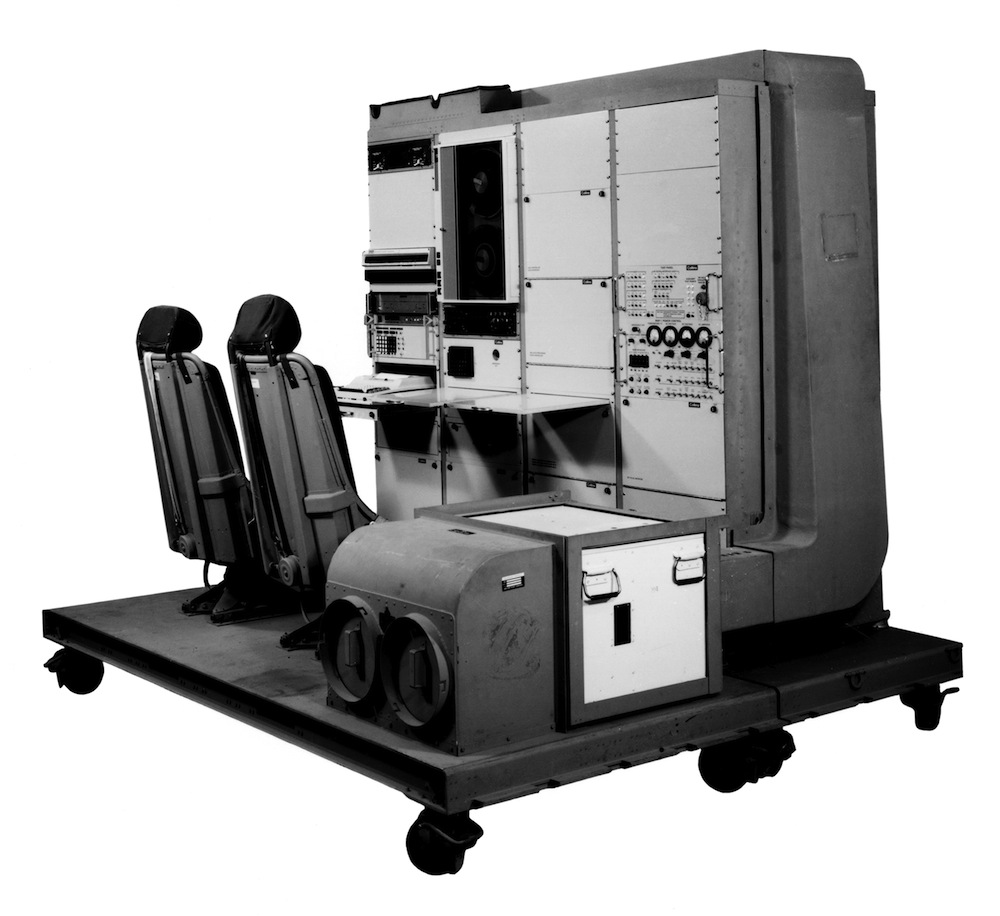
\includegraphics[width=\textwidth]{images/erster_empfaenger.jpg}
            \end{figure}
            \centering{\small [TimeAndNavigation]}
        \end{column}\pause
        \begin{column}{0.5\textwidth}
            Verladung des ersten GPS III Satelliten
            \begin{figure}
                \centering
                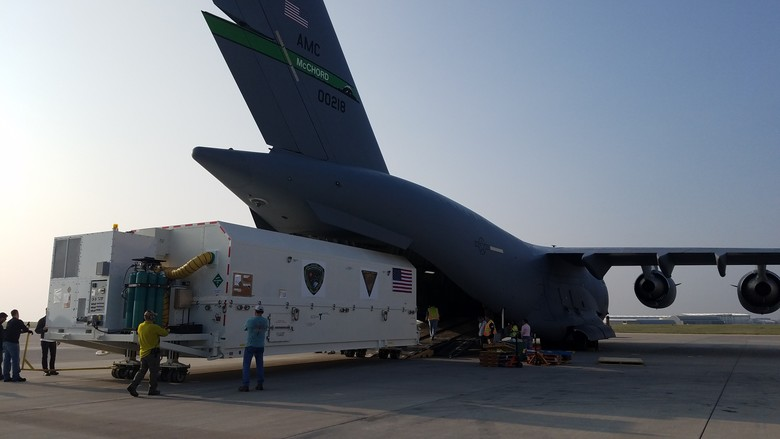
\includegraphics[width=\textwidth]{images/gps3-satellit-verladung.JPG}
            \end{figure}
            {\small [gps.gov]}
        \end{column}
    \end{columns}
\end{frame}

\begin{frame}{Aussichten}
    \begin{figure}
        \centering
        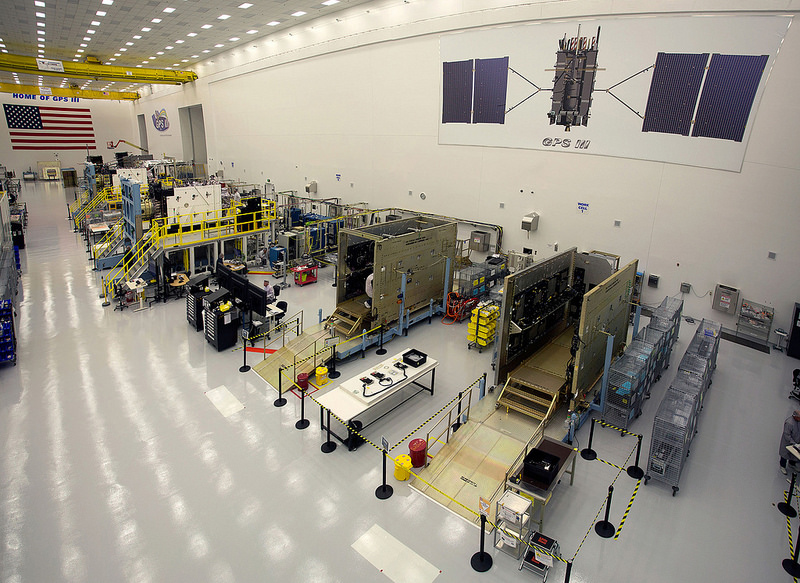
\includegraphics[height=0.85\textheight]{images/gps-3-construction.jpg}
    \end{figure}
    ~\centering{\small [lockheedmartin.com]}
\end{frame}

\section{Nicht behandelte Themengebiete}
\begin{frame}{Nicht behandelte Themengebiete}
    \begin{itemize}
        \item Genaue Bestimmung der Satellitenorbits
        \item Koordinatentransformationen
        \item Nutation \& Präzession der Erde
        \item Zeittransformationen
    \end{itemize}
\end{frame}
